\documentclass[14pt]{extbook}
\usepackage{multicol, enumerate, enumitem, hyperref, color, soul, setspace, parskip, fancyhdr} %General Packages
\usepackage{amssymb, amsthm, amsmath, bbm, latexsym, units, mathtools} %Math Packages
\everymath{\displaystyle} %All math in Display Style
% Packages with additional options
\usepackage[headsep=0.5cm,headheight=12pt, left=1 in,right= 1 in,top= 1 in,bottom= 1 in]{geometry}
\usepackage[usenames,dvipsnames]{xcolor}
\usepackage{dashrule}  % Package to use the command below to create lines between items
\newcommand{\litem}[1]{\item#1\hspace*{-1cm}\rule{\textwidth}{0.4pt}}
\pagestyle{fancy}
\lhead{Progress Quiz 1}
\chead{}
\rhead{Version A}
\lfoot{3735-1698}
\cfoot{}
\rfoot{Spring 2021}
\begin{document}

\begin{enumerate}
\litem{
Write the equation of the line in the graph below in Standard form $Ax+By=C$. Then, choose the intervals that contain $A, B, \text{ and } C$.
\begin{center}
    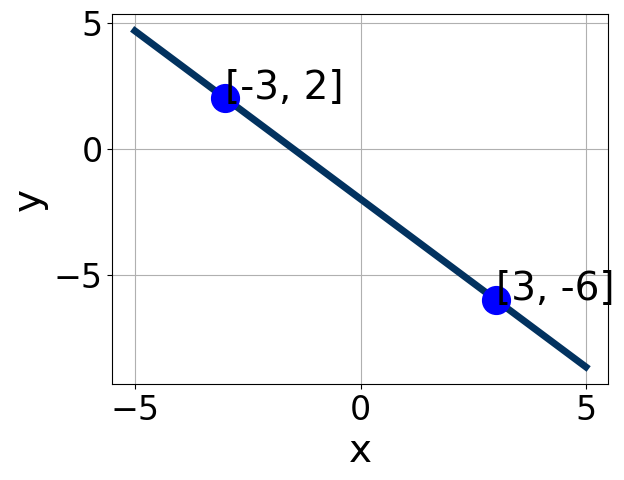
\includegraphics[width=0.5\textwidth]{../Figures/linearGraphToStandardA.png}
\end{center}
\begin{enumerate}[label=\Alph*.]
\item \( A \in [1.9, 9.1], \hspace{3mm} B \in [-2.93, -1.9], \text{ and } \hspace{3mm} C \in [9.5, 11.3] \)
\item \( A \in [-4.5, -1.5], \hspace{3mm} B \in [0.93, 1.87], \text{ and } \hspace{3mm} C \in [-6.3, -3.6] \)
\item \( A \in [-5.6, -3.6], \hspace{3mm} B \in [1.99, 2.33], \text{ and } \hspace{3mm} C \in [-12.1, -9.9] \)
\item \( A \in [-4.5, -1.5], \hspace{3mm} B \in [-1.01, -0.52], \text{ and } \hspace{3mm} C \in [3.8, 5.3] \)
\item \( A \in [1.9, 9.1], \hspace{3mm} B \in [1.99, 2.33], \text{ and } \hspace{3mm} C \in [-12.1, -9.9] \)

\end{enumerate} }
\litem{
Write the equation of the line in the graph below in Standard form $Ax+By=C$. Then, choose the intervals that contain $A, B, \text{ and } C$.
\begin{center}
    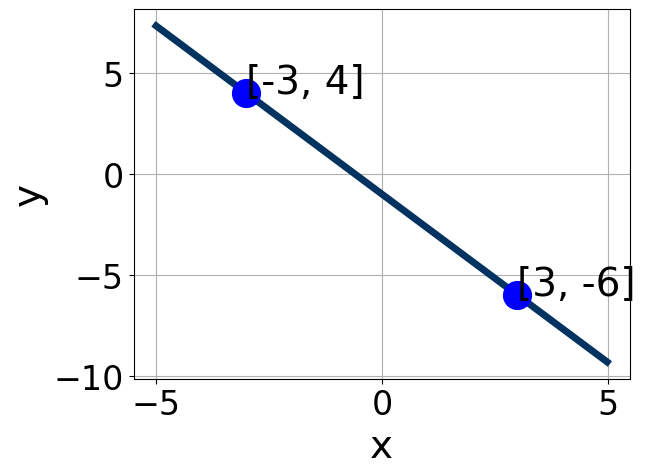
\includegraphics[width=0.5\textwidth]{../Figures/linearGraphToStandardCopyA.png}
\end{center}
\begin{enumerate}[label=\Alph*.]
\item \( A \in [1.82, 4.08], \hspace{3mm} B \in [1.6, 5.7], \text{ and } \hspace{3mm} C \in [-33, -23] \)
\item \( A \in [-1.02, 0.23], \hspace{3mm} B \in [0.6, 1.7], \text{ and } \hspace{3mm} C \in [-5, -1] \)
\item \( A \in [-3.33, -1.68], \hspace{3mm} B \in [1.6, 5.7], \text{ and } \hspace{3mm} C \in [-33, -23] \)
\item \( A \in [-1.02, 0.23], \hspace{3mm} B \in [-2, 0.1], \text{ and } \hspace{3mm} C \in [-1, 6] \)
\item \( A \in [1.82, 4.08], \hspace{3mm} B \in [-5.1, -3.2], \text{ and } \hspace{3mm} C \in [23, 30] \)

\end{enumerate} }
\litem{
Find the equation of the line described below. Write the linear equation as $ y=mx+b $ and choose the intervals that contain $m$ and $b$.\[ \text{Perpendicular to } 5 x + 6 y = 15 \text{ and passing through the point } (6, 8). \]\begin{enumerate}[label=\Alph*.]
\item \( m \in [0.31, 1.12] \hspace*{3mm} b \in [0.4, 1.6] \)
\item \( m \in [1.13, 2.89] \hspace*{3mm} b \in [-1.2, 0.6] \)
\item \( m \in [-1.53, -0.91] \hspace*{3mm} b \in [12.4, 15.9] \)
\item \( m \in [1.13, 2.89] \hspace*{3mm} b \in [1.6, 4.4] \)
\item \( m \in [1.13, 2.89] \hspace*{3mm} b \in [0.4, 1.6] \)

\end{enumerate} }
\litem{
First, find the equation of the line containing the two points below. Then, write the equation as $ y=mx+b $ and choose the intervals that contain $m$ and $b$.\[ (-10, -8) \text{ and } (-7, 7) \]\begin{enumerate}[label=\Alph*.]
\item \( m \in [5, 6] \hspace*{3mm} b \in [13, 19] \)
\item \( m \in [5, 6] \hspace*{3mm} b \in [41, 45] \)
\item \( m \in [-7, -2] \hspace*{3mm} b \in [-35, -26] \)
\item \( m \in [5, 6] \hspace*{3mm} b \in [-46, -39] \)
\item \( m \in [5, 6] \hspace*{3mm} b \in [1, 8] \)

\end{enumerate} }
\litem{
Solve the equation below. Then, choose the interval that contains the solution.\[ -19(2x -9) = -7(-15x + 16) \]\begin{enumerate}[label=\Alph*.]
\item \( x \in [-0.64, 0.02] \)
\item \( x \in [0.2, 0.62] \)
\item \( x \in [-0.96, -0.79] \)
\item \( x \in [1.54, 2.19] \)
\item \( \text{There are no real solutions.} \)

\end{enumerate} }
\litem{
Find the equation of the line described below. Write the linear equation as $ y=mx+b $ and choose the intervals that contain $m$ and $b$.\[ \text{Perpendicular to } 5 x + 4 y = 14 \text{ and passing through the point } (5, -10). \]\begin{enumerate}[label=\Alph*.]
\item \( m \in [-0.86, -0.35] \hspace*{3mm} b \in [-7.11, -4.81] \)
\item \( m \in [0.91, 1.81] \hspace*{3mm} b \in [-14.05, -13.3] \)
\item \( m \in [0.41, 1.11] \hspace*{3mm} b \in [-14.05, -13.3] \)
\item \( m \in [0.41, 1.11] \hspace*{3mm} b \in [13.34, 14.87] \)
\item \( m \in [0.41, 1.11] \hspace*{3mm} b \in [-15.08, -14.34] \)

\end{enumerate} }
\litem{
Solve the equation below. Then, choose the interval that contains the solution.\[ -14(13x + 12) = -3(15x + 2) \]\begin{enumerate}[label=\Alph*.]
\item \( x \in [-1.27, -1.05] \)
\item \( x \in [-0.86, -0.75] \)
\item \( x \in [1.26, 1.29] \)
\item \( x \in [-1.3, -1.22] \)
\item \( \text{There are no real solutions.} \)

\end{enumerate} }
\litem{
Solve the linear equation below. Then, choose the interval that contains the solution.\[ \frac{-6x -7}{5} - \frac{6x + 5}{8} = \frac{-7x -5}{4} \]\begin{enumerate}[label=\Alph*.]
\item \( x \in [-5.88, -0.88] \)
\item \( x \in [-1.16, 0.84] \)
\item \( x \in [0.38, 5.38] \)
\item \( x \in [-37, -31] \)
\item \( \text{There are no real solutions.} \)

\end{enumerate} }
\litem{
First, find the equation of the line containing the two points below. Then, write the equation as $ y=mx+b $ and choose the intervals that contain $m$ and $b$.\[ (-4, -8) \text{ and } (5, -10) \]\begin{enumerate}[label=\Alph*.]
\item \( m \in [-0.35, -0.06] \hspace*{3mm} b \in [-4.5, -1.3] \)
\item \( m \in [-0.14, 0.49] \hspace*{3mm} b \in [-12.8, -9.9] \)
\item \( m \in [-0.35, -0.06] \hspace*{3mm} b \in [-10.9, -8.8] \)
\item \( m \in [-0.35, -0.06] \hspace*{3mm} b \in [-18.1, -14.9] \)
\item \( m \in [-0.35, -0.06] \hspace*{3mm} b \in [7.5, 10.5] \)

\end{enumerate} }
\litem{
Solve the linear equation below. Then, choose the interval that contains the solution.\[ \frac{5x -4}{7} - \frac{-4x + 5}{4} = \frac{3x -7}{2} \]\begin{enumerate}[label=\Alph*.]
\item \( x \in [-8.83, -4.83] \)
\item \( x \in [-21.5, -17.5] \)
\item \( x \in [-1.28, 0.72] \)
\item \( x \in [9.33, 11.33] \)
\item \( \text{There are no real solutions.} \)

\end{enumerate} }
\end{enumerate}

\end{document}